\section{Questions sur le chapitre ``L'air humide''}
\subsection{Pourquoi lorsque l'on projette dans l'air de l'eau en fines gouttelettes, la température diminue ?}
Lorsque l'on projette de l'eau en fines gouttelettes, l'air va capter de l'humidité jusqu'à ce que $\phi=1$ en suivant une isenthalpique. On peut voir sur le diagramme de l'air humide qu'augmenter l'humidité relative par un procédé isenthalpique diminue la température. 

\subsection{Pourquoi peut-on considérer l'air humide comme un gaz parfait ?}
On peut considérer l'air humide comme un gaz parfait étant donné que la pression partielle de l'eau est nettement plus basse que la pression atmosphérique :
\begin{equation} p_{H_20} = \SI{18.23}{\kilo\pascal} \ll p_\text{atm} = \SI{101.325}{\kilo\pascal} \end{equation}
De plus, l'air humide contenant très peu d'eau, il peut être considéré comme un gaz parfait. Quand la pression tend vers zéro, tous les gaz sont considérés comme parfaits. 

\subsection{Comment fonctionne une tour de refroidissement ? Dans quelles conditions fontionne-t-elle le plus efficacement ?}
L'eau chauffée dans le condenseur jusqu'à la température $t_s$ et d'un débit massique $\dot{m}_e$ est dispersée sur un ensemble de plaques verticales. L'eau est de ce fait mise en contact avec une masse d'air froid, ascendante, de débit $\dot{m}_{as}$ d'air sec entrant au pied de la tour et caractérisée par l'état 1 (voir Figure \ref{fig:tour_de_refroidissement}. Il est à noter que ce débit résulte uniquement du tirage naturel créé par l'échauffement de l'air dans la tour. Un transfert de masse et de chaleur s'établit entre l'air et l'eau. L'eau se refroidit et s'évapore en partie. L'air se réchauffe et s'humidifie. Deux bilans peuvent être établis pour la conservation de la masse :
\begin{itemize}
	\item Conservation du débit d'air sec;
	\item Conservation du débit d'eau : l'eau évaporée correspond à l'augmentation d'humidité dans l'air.
\end{itemize}
\begin{figure}[h]\centering
	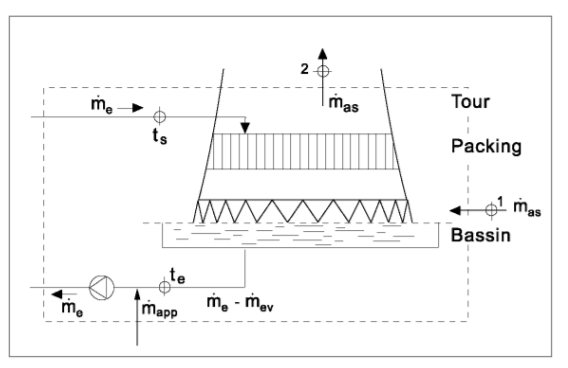
\includegraphics[width=0.6\textwidth]{figures/tour_de_refroidissement.png}
	\caption{Tour de refroidissement}
	\label{fig:tour_de_refroidissement}
\end{figure}

\subsection{Définissez l'humidité absolue et l'humidité relative. Expliquez aussi le lien entre les deux.}
L'humidité absolue, notée $x_v$, est la quantité massique de vapeur d'eau contenue dans l'air humide par quantité massique d'air sec :
\begin{equation} x_v = \frac{M_{H_2O}}{M_\text{air sec}}\frac{p_{H_2O}}{p-p_{H_2O}} \end{equation}
L'humidité relative, notée $\phi$, est le rapport entre la quantité volumique ou molaire de vapeur d'eau dans l'air humide à la température considérée et la quantité maximale que pourrait contenir l'air humide à cette même température (s'il était saturé) :
\begin{equation} \phi = \frac{p_{H_2O}}{p_\text{sat}(t)} \end{equation}
Les deux humidités sont liées par l'équation :
\begin{equation} x_v = \frac{M_{H_2O}}{M_\text{air sec}}\frac{\phi p_\text{sat}(t)}{p-\phi p_\text{sat}(t)} \end{equation}

\subsection{Expliquez le principe de fonctionnement d'un séchoir.}
Le principe est assez simple. Il s’agit premièrement de faire chauffer de l’air humide. En le faisant chauffer, son humidité relative $\phi$ diminue tandis que son humidité absolue x reste constante. Ensuite on établit un contact direct entre cet air humide chauffé et le linge afin d’évaporer l’humidité présente dans le linge. Au contact entre l’air humide chaud et le linge, l’air chaud va capter l’humidité du linge jusqu’à un état saturé $\phi = 1$. L’air chargé d’humidité passe sur un condenseur (à air) qui transforme l’humidité en eau. (Il y a un contact entre cet air chaud et de l’air froid. L’humidité relative diminue et l’air se dégorge de son eau). Celle-ci est stockée dans un bac, situé de préférence en haut de l’appareil, qu’il suffit de vider régulièrement.

\subsection{Expliquez le fonctionnement d'un canon à neige.}
La neige artificielle est créée en pulvérisant finement de l’eau dans de l’air sec. Le mélange adiabatique des deux éléments induit un refroidissement global de l’air et de l’eau et aboutit à la formation de cristaux de glace. Pour obtenir de la neige, il faut un mélange à une température inférieure à \SI{0}{\celsius}. Pour se faire, si on réfléchis intuitivement avec le diagramme de l’air humide, il faut non seulement être à une température basse mais il doit aussi être relativement sec. Si l’air vaporise plus d’eau, alors sa température va diminuer encore plus. L’air va vaporiser plus d’eau s’il est bien sec, donc il faut un air relativement sec et froid. 

Il est donc plus aisé de créer de la neige artificielle avec de l’air à une température de \SI{5}{\celsius} et une faible humidité relative que de la créer dans de l’air à \SI{2}{\celsius} mais à la limite de la saturation.

Après pulvérisation de l’eau, l’air est à saturation et a une température légèrement inférieure à \SI{0}{\celsius}. Si on continue à pulvériser de l’eau sur l’air qui est déjà saturé et à température inférieure à \SI{0}{\celsius}, alors il y aura formation de neige.

La pression a également une influence sur la formation de neige. Plus la pression est basse, plus il est facile d’obtenir de la neige. Penser qu’en haut du mont blanc la pression est de \SI{54}{\kilo\pascal} et qu’il fait tout blanc là bas.
